\ifdefined\XeTeXrevision\else\pdfoutput=1\fi
\documentclass[11pt]{article}
\usepackage[margin=1in]{geometry}
\usepackage{graphicx}
\usepackage{booktabs}
\usepackage{amsmath}
\usepackage{amssymb}
\usepackage{xcolor}
\usepackage{hyperref}
\usepackage{microtype}
\emergencystretch=2em  % long \texttt{} run names would otherwise overflow the margin
\hypersetup{
  colorlinks=true,
  linkcolor=blue!60!black,
  citecolor=blue!60!black,
  urlcolor=blue!60!black,
  pdftitle={Zero Weight-Space Interference Is Not Enough},
  pdfauthor={Franci Penov},
}
\graphicspath{{figures/}}
\title{Zero Weight-Space Interference Is Not Enough:\\Behavioral Probes for Composing Sensor Bricks\\on a Frozen Language Model}
\author{Franci Penov \\ kortexa.ai \\ \texttt{francip@kortexa.ai}}
\date{2026-08-03}

\begin{document}
\maketitle

\begin{abstract}
Modular adaptation promises that separately trained sensor adapters can be merged into one model that serves all of them. The standard evidence for a successful merge is an in-objective metric --- perplexity, bits-per-byte, or a single downstream score. We argue that such metrics certify nothing, and we build the instrument they are missing: each constituent's own out-of-objective behavioral probe, re-measured under the merged weights. On a frozen 230M-parameter language model with three sensor bricks (IMU, audio, vision) generated by conditional LoRA bridges, the instrument immediately separates the two: the merge with the best bits-per-byte retention we have ever recorded (94.7\%) has behaviorally dead probes, indistinguishable from the merge that scores -106.5\%. With that instrument we report an exhaustive negative on additive composition. Allocating each brick a disjoint block of a shared frozen orthonormal basis makes the merge provably lossless --- projecting the merged delta back onto a brick's own block recovers its coefficients at ratio 1.000006 --- and it buys nothing: across three seeds, two allocations, and four merge rules spanning a 3$\times$ range of norms, a six-way IMU probe worth 0.724 alone is worth 0.135 merged against a 0.167 chance rate, and a powered fifty-way audio probe worth 0.297 alone scores 0.000. One foreign brick is as damaging as two, and a continuous dose-response shows the 80\% retention gate is met only when foreign bricks are attenuated to $\cos \approx 0.99$ --- about 7 degrees of tolerance. We then falsify our own mechanism: partitioning \emph{layers} instead of coefficients gives each brick perfect ownership of its sites ($\cos = 0.9999999$ in-block, zero foreign mass in-block) and retention is still 4.5--32.6\%, replicated at two seeds, with the merged probe equal to deleting the measured brick. The damage is cross-layer residual-stream interaction, not weight-space overlap. Finally, selection works where addition cannot: an oracle router recovers every brick's single-brick probe exactly (16/16 cells at 8 seeds), and a task-conditioned learned router reaches that ceiling exactly when it escapes a collapse basin --- which it does in 6 seeds of 8, with no hyperparameter predicting which. We state the resulting open problem: make the escape selectable.
\end{abstract}

\section{Introduction}
A conditional LoRA bridge \cite{penov2026bridges} maps a frozen sensor encoder's features to per-input low-rank weight updates injected into a frozen language model, giving the model token-free awareness of an external signal. A follow-up study \cite{penov2026basis} reparameterized the bridge's output as $k$ coefficients over a basis of LoRA directions, and proved that coefficient-space composition is \emph{identical} to weight-space composition, since $\mathrm{mean}(c_i \cdot B) = \mathrm{mean}(c_i) \cdot B$. That located the failure in the merge operation and named an untested fix: give each modality its own block of a shared frozen orthonormal basis, so that weight-space interference is zero by construction. This paper runs that experiment, and everything the experiment forced afterwards.

The result is a negative, and the reason it is worth reporting is methodological. One claim connects this paper to its predecessors:

\begin{quote}
A metric computed in the space the intervention was optimized in certifies nothing. Certification requires an out-of-objective behavioral probe.
\end{quote}

Composition research is unusually exposed to this. Bits-per-byte, perplexity, and averaged benchmark scores are cheap to compute under a merge and they move for reasons that have nothing to do with whether the merged model can still \emph{do} what each constituent could do. Section~\ref{sec:instrument} makes that concrete in one table: the merge with the highest BPB retention in this program is behaviorally dead, and it is dead in exactly the same way as the merge with the worst BPB retention.

\paragraph{Contributions.}
\begin{itemize}
  \item \textbf{An instrument} (\S\ref{sec:instrument}): each constituent's own task probe re-measured under merged weights, against its single-brick score, the published feature controls, and an \texttt{others\_only} control that zeroes the measured brick inside the merge. Instantiated by an anti-metric result --- 94.7\% BPB retention on probes at chance.
  \item \textbf{An exhaustive additive negative} (\S\ref{sec:negative}): provably lossless disjoint-sum composition is behaviorally dead across three seeds, two allocations and four merge rules; damage is presence-driven rather than count-driven, graded by angle, and a controlled dose-response bounds the tolerance at roughly 7 degrees.
  \item \textbf{A mechanism, correctly localized} (\S\ref{sec:mechanism}): a layer-partitioned design that our own angle account predicted would retain $\sim$100\% instead retains 4.5--32.6\%, replicated at two seeds. The interference is cross-layer and downstream, not in the weights.
  \item \textbf{Selection, honestly} (\S\ref{sec:selection}): the routing ceiling is exact at every seed; the only learned mechanism that reaches it is bistable across seeds and must be handed the task identity. We report the escape rate rather than a method.
\end{itemize}

\section{Setup}
\label{sec:setup}
\paragraph{Model and bricks.}
The base model is LiquidAI LFM~2.5 230M, frozen, adapted through the published harness's HuggingFace checkpoint path \cite{penov2026note}. LoRA rank 4 on attention and MLP projections gives a flattened adaptation vector of $D = 774,144$ dimensions. Three bricks are trained, each alone, by the ordinary recipe: two \emph{task} bricks with closed-set ranking probes --- IMU (6-way activities, chance 0.167) and audio (50-way events, chance 0.020) --- and one \emph{context} brick (vision) trained on the text objective, which has no label probe in this suite and therefore enters only through the damage it does. Trainable parameters per brick: 181,120 (IMU), 197,504 (audio).

\paragraph{Shared frozen basis and allocations.}
Each brick's bridge emits $k$ coefficients over a shared frozen orthonormal basis $B \in \mathbb{R}^{k \times D}$, built by Cholesky whitening of a seeded Gaussian ($\max |BB^\top - I|$ off-diagonal $\le 4.7e-08$ at $k = 768$). The basis is a buffer, not a parameter: it is regenerated from its seed and never stored. Three allocations are compared. Under \textbf{shared} allocation all bricks write all $k$ rows. Under \textbf{disjoint} allocation brick $i$ writes only rows $[i \cdot k/n, (i{+}1) \cdot k/n)$, so no two bricks ever touch the same coordinate. Under \textbf{layer} allocation (\S\ref{sec:mechanism}) each brick gets its own basis over its own contiguous block of decoder layers.

\paragraph{Merge rules.}
\texttt{sum} adds every brick's delta; \texttt{mean} averages them; \texttt{alpha-norm} rescales the sum per item so its $L_2$ matches that item's own single-brick delta norm; \texttt{alpha-rsqrtn} is the variance-preserving $1/\sqrt{n}$ point; \texttt{beta-}$\beta$ applies $\mathrm{own} + \beta \cdot \mathrm{others}$, so $\beta = 1$ is exactly \texttt{sum}. The gated modes of \S\ref{sec:selection} apply a convex weight per brick, so a confident gate reproduces a single brick exactly and a uniform gate reproduces \texttt{mean}.

\paragraph{Budgets and slice width.}
Table~\ref{tab:pilot} sets the per-modality slice width from single-modality frozen probes. IMU is far stronger at width 256 than at 128 and audio is marginally better, so three modalities $\times$ 256 rows fixes $k_{\mathrm{total}} = 768$; the shared arm uses $k = 256$, which by prefix-stability of Cholesky whitening is literally the first 256 rows of the same basis. Budgets are the house standard: learning rate $10^{-3}$, 32{,}768 evaluation tokens, 64 stratified evaluation items per probe, 600 task steps for IMU and 300 text steps for vision. Audio at 600 steps is underpowered (Table~\ref{tab:pilot}); the registered fix is 1800 steps, which lifts a single audio brick from 0.078 to 0.328 against a 0.016 no-bridge baseline. Every behavioral claim below is scoped to the two \emph{powered} probes: IMU at 600 steps and audio at 1800. Vision was never powered as a probe and no behavioral claim is made about it.

\begin{table}[t]
\centering
\caption{Single-modality frozen-basis probes that fix the slice width and the audio budget. Rank-1 accuracy, \texttt{true} condition; all controls sit at chance in every frozen run.}
\label{tab:pilot}
\begin{tabular}{lrrrr}
\toprule
Probe & Slice width & Steps & Rank-1 & Chance \\
\midrule
IMU (6-way) & 128 & 600 & 0.484 & 0.167 \\
IMU (6-way) & 256 & 600 & 0.750 & 0.167 \\
Audio (50-way) & 128 & 600 & 0.062 & 0.020 \\
Audio (50-way) & 256 & 600 & 0.078 & 0.020 \\
Audio (50-way) & 256 & 1800 & 0.328 & 0.020 \\
\bottomrule
\end{tabular}
\end{table}

\paragraph{Statistical hygiene.}
Every probe is a closed-set ranking probe over 64 stratified evaluation items, so one item is 1.6 points. The 95\% binomial half-width at the six-way chance rate is $\pm0.091$ and at the fifty-way rate $\pm0.034$. We never rank cells inside those bands: a merged IMU score anywhere between roughly 0.08 and 0.26 is ``at chance'' and its exact value carries no information. This is why the registered gate is set at 80\% retention rather than at 95\%, and why the paper leans on three-seed aggregates, eight-seed rates, and the dose curve rather than on individual cells. Cells that rest on a single seed are labelled as such in every table and in the text.

\paragraph{The registered gate.}
Stated before any run: composition is \emph{supported} only if \textbf{every} measured task modality retains $\ge 80\%$ of that same brick's single-brick rank-1 under the merge, with the \texttt{shuffled} / \texttt{random} / \texttt{no\_bridge} controls at chance. A cell where one modality clears and the other does not is a failure. This roll-up rule is unchanged across every arm in the paper.

\section{The instrument, and why the usual metric is not one}
\label{sec:instrument}
The composition instrument re-measures \emph{each brick's own probe under the merged weights}. Every cell is reported against four references: that brick's single-brick score, the published \texttt{shuffled} and \texttt{random} feature controls, \texttt{no\_bridge}, and --- the load-bearing one --- \texttt{others\_only}, which zeroes the measured brick's delta inside the merge and leaves the others. \texttt{others\_only} answers the question a retention percentage cannot: is the brick's contribution \emph{diluted}, or is it \emph{inaudible}?

Table~\ref{tab:bpb} is the reason the instrument had to be built. It reports bits-per-byte retention for the same three bricks merged four ways, beside the IMU task probe measured on the identical merges. BPB retention tracks exactly one thing --- how close the merged delta's norm lands to a single brick's --- and it orders the merges in a way that is not merely uninformative but actively inverted. Shared-plus-sum is the best composition BPB number this program has recorded; it gets there because a shared basis lets three coefficient vectors overlap so their sum stays near single-brick scale (21.7 against a single brick's 19.0) instead of growing orthogonally to 33.2, which is precisely what disjointness forces. And that ``winning'' merge has the same extinguished task probe as the merge that scores -106.5\%: IMU 0.141 against 0.141, both at the 0.167 chance rate.

\begin{table}[t]
\centering
\caption{The anti-metric result. BPB retention on the merged bricks (secondary metric, computed in the training objective) against the IMU task probe measured on the same merges (out-of-objective). A metric on which the behaviorally dead configuration scores 94.7\% is not measuring composition. Single seed (42).}
\label{tab:bpb}
\small
\begin{tabular}{lrrrrr}
\toprule
Merge & $\|\Delta_{\mathrm{merged}}\|$ & $\Delta$BPB & BPB retention & IMU rank-1 & IMU retention \\
\midrule
shared + \texttt{mean} & 7.2 & +0.0102 & 24.6\% & 0.172 & 25.6\% \\
disjoint + \texttt{mean} & 11.1 & +0.0220 & 53.0\% & 0.172 & 22.9\% \\
shared + \texttt{sum} & 21.7 & +0.0392 & 94.7\% & 0.141 & 20.9\% \\
disjoint + \texttt{sum} & 33.2 & -0.0442 & -106.5\% & 0.141 & 18.8\% \\
\bottomrule
\end{tabular}
\end{table}

\section{The additive negative}
\label{sec:negative}

\subsection{The construction delivers, and it buys nothing}
Disjoint allocation was designed to make weight-space interference zero, and it does, measurably. Projecting the merged delta back onto a brick's own block of the basis recovers that brick's coefficients at ratio 1.000006 with relative error 5.7e-06 under \texttt{sum} --- zero cross-terms and zero dilution --- against ratio 1.090 at relative error 0.90 for the shared arm, which is thoroughly contaminated. Under \texttt{mean} the same projection returns exactly $1/n$ (0.33334), reproducing the dilution mechanism of prior work to four decimals. The norms confirm orthogonality independently: in the disjoint arm $\sqrt{\|{\mathrm{own}}\|^2 + \|{\mathrm{others}}\|^2} = \sqrt{52.59^2 + 50.33^2} = 72.79 = \|{\mathrm{sum}}\|$ exactly, while in the shared arm 70.89 $\ne$ 74.63.

It buys nothing. Table~\ref{tab:seeds} gives three seeds of each allocation on the powered IMU probe. A brick worth 0.724 $\pm$ 0.023 alone is worth 0.135 $\pm$ 0.055 inside the three-way sum, against chance 0.167: retention 18.6\%. The shared arm --- whose weight space is contaminated --- lands in the same place, 22.3\%. Every seed of every arm is at or below chance, and the spread across seeds is roughly a fifth of the distance to the gate. The probe is not degraded; it is extinguished, and the two arms are indistinguishable, which is the whole point: weight-space cleanliness is measurable, achievable, and behaviorally inert.

The \texttt{others\_only} control says what kind of failure this is. Deleting the measured brick from the merge entirely scores 0.156 (IMU) and 0.016 (audio) against merged scores of 0.109 and 0.000. The brick's contribution is not diluted; it is inaudible.

\begin{table}[t]
\centering
\caption{Three seeds (42, 1042, 2042) of each allocation on the six-way IMU probe, mean $\pm$ half-spread. Chance is 0.167; the 95\% binomial half-width is $\pm0.091$. All controls at chance in every run.}
\label{tab:seeds}
\begin{tabular}{llrrr}
\toprule
Allocation & Merge & Single rank-1 & Merged rank-1 & Retention \\
\midrule
disjoint-768 & sum & 0.724 $\pm$ 0.023 & 0.135 $\pm$ 0.055 & 18.6\% $\pm$ 7.5\% \\
disjoint-768 & mean & 0.724 $\pm$ 0.023 & 0.167 $\pm$ 0.008 & 23.0\% $\pm$ 0.8\% \\
shared-256 & sum & 0.703 $\pm$ 0.031 & 0.156 $\pm$ 0.055 & 22.3\% $\pm$ 8.1\% \\
shared-256 & mean & 0.703 $\pm$ 0.031 & 0.177 $\pm$ 0.008 & 25.2\% $\pm$ 0.6\% \\
\bottomrule
\end{tabular}
\end{table}

\subsection{Magnitude is excluded}
Four merge rules on the same trained bricks span a 3$\times$ range of merged norms, including one (\texttt{alpha-norm}) that matches the measured brick's own norm to four decimals (52.59 against $\|\mathrm{own}\| = 52.59$). None recovers anything (Table~\ref{tab:merges}). The reason is in one column: all four are positive rescalings of the same vector, so all four share one $\cos(\mathrm{merged}, \mathrm{own})$. Magnitude was the only thing they varied, and magnitude does not matter. What is left is direction.

\begin{table}[t]
\centering
\caption{Four merge rules, one set of trained bricks, seed 42 (single seed). All four are positive rescalings of the same merged direction, so $\cos$ is shared; the norms span 3$\times$ and the probes are dead in all of them. Chance: IMU 0.167, audio 0.020.}
\label{tab:merges}
\small
\begin{tabular}{lrrrrrr}
\toprule
Merge & $\|\Delta_{\mathrm{merged}}\|$ & $\cos(\mathrm{merged}, \mathrm{own})$ & IMU rank-1 & IMU ret. & Audio rank-1 & Audio ret. \\
\midrule
\texttt{mean} & 24.06 & 0.7287 & 0.172 & 22.9\% & 0.016 & 5.3\% \\
\texttt{alpha-rsqrtn} & 41.67 & 0.7287 & 0.125 & 16.7\% & 0.016 & 5.3\% \\
\texttt{alpha-norm} & 52.59 & 0.7287 & 0.156 & 20.8\% & 0.016 & 5.3\% \\
\texttt{sum} & 72.17 & 0.7287 & 0.109 & 14.6\% & 0.000 & 0.0\% \\
\bottomrule
\end{tabular}
\end{table}

\subsection{Presence, not count --- and the angle grades it}
Halving the number of foreign bricks changes nothing (Table~\ref{tab:pairwise}): audio goes to 0.000 with one foreign brick and 0.000 with two; IMU retains 15.9\% against 14.6\%. One foreign brick is as fatal as two. What does move the number is the angle the foreign bricks open, which is set by their norm relative to the measured brick's: the small vision context brick ($\|\Delta\| \approx 18.9$ against IMU's $53.2$) leaves IMU at 36.4\% where audio leaves it at 15.9\%. Both modalities order the same way, and the covariate that predicts retention is $\cos$, not brick count. These rows are single-seed and are read as an ordering, not as point estimates.

\begin{table}[t]
\centering
\caption{Damage against the number of foreign bricks and against the angle they open, sum merge, seed 42 (single seed), identical per-brick budgets. Retention is against each modality's own single-brick rank-1 in the same run.}
\label{tab:pairwise}
\small
\begin{tabular}{llrrrrrrr}
\toprule
Measured & Foreign & \# & $\cos(\mathrm{sum}, \mathrm{own})$ & $\|\mathrm{own}\|$ & $\|\mathrm{others}\|$ & Single & Merged & Retention \\
\midrule
imu & audio & 1 & 0.7688 & 53.2 & 44.2 & 0.688 & 0.109 & 15.9\% \\
imu & vision & 1 & 0.9421 & 53.2 & 18.9 & 0.688 & 0.250 & 36.4\% \\
imu & audio + vision & 2 & 0.7287 & 52.6 & 49.4 & 0.750 & 0.109 & 14.6\% \\
audio & imu & 1 & 0.6395 & 44.2 & 53.2 & 0.297 & 0.000 & 0.0\% \\
audio & vision & 1 & 0.9319 & 48.6 & 18.9 & 0.391 & 0.078 & 20.0\% \\
audio & imu + vision & 2 & 0.6324 & 45.6 & 55.9 & 0.297 & 0.000 & 0.0\% \\
\bottomrule
\end{tabular}
\end{table}

\subsection{The dose-response}
Comparing brick sets confounds ``how many foreign bricks'' with ``how large are they'', so the \texttt{beta-}$\beta$ merge attenuates the foreign contribution continuously and sweeps $\cos(\mathrm{merged}, \mathrm{own})$ with everything else held fixed. This is the paper's central measurement (Table~\ref{tab:dose}, Figure~\ref{fig:dose}). The registered 80\% gate is met only at $\beta = 0.125$, i.e. $\cos \approx 0.99$, i.e. with the foreign bricks attenuated to an eighth of their trained strength --- and even there only for IMU; the fifty-way audio probe is already down to 63.2\%. A brick tolerates roughly 7 degrees of rotation of its adaptation before it starts losing its probe, and by 25 degrees it has lost about two thirds of it.

Two consequences. First, \emph{no additive rule can work}: at $\beta = 1$ every brick contributes at full strength by definition, and the curve is already on the floor. Second, the curve does not say composition is impossible --- it says the other bricks have to be \emph{muted}, which is a description of selection rather than of arithmetic. This single run is seed 42; the ordering it establishes is corroborated by the pairwise arm and by the three-seed table, but the curve itself is not replicated.

\begin{table}[t]
\centering
\caption{Dose-response: retention against $\cos(\mathrm{merged}, \mathrm{own})$ under $\mathrm{own} + \beta \cdot \mathrm{others}$, seed 42 (single seed). $\beta = 1$ is \texttt{sum}; $\beta = 0$ would be the single brick. Angles are for IMU. Retention is against singles of 0.750 (IMU) and 0.297 (audio).}
\label{tab:dose}
\begin{tabular}{rrrrrr}
\toprule
$\beta$ & $\cos$ (IMU) & angle & IMU retention & $\cos$ (audio) & Audio retention \\
\midrule
0.125 & 0.993 & 6.7$^\circ$ & 100.0\% & 0.988 & 63.2\% \\
0.25 & 0.973 & 13.2$^\circ$ & 72.9\% & 0.956 & 26.3\% \\
0.5 & 0.905 & 25.2$^\circ$ & 37.5\% & 0.853 & 5.3\% \\
0.75 & 0.817 & 35.2$^\circ$ & 14.6\% & 0.736 & 10.5\% \\
1 & 0.729 & 43.2$^\circ$ & 14.6\% & 0.632 & 0.0\% \\
\bottomrule
\end{tabular}
\end{table}

\begin{figure}[t]
\centering
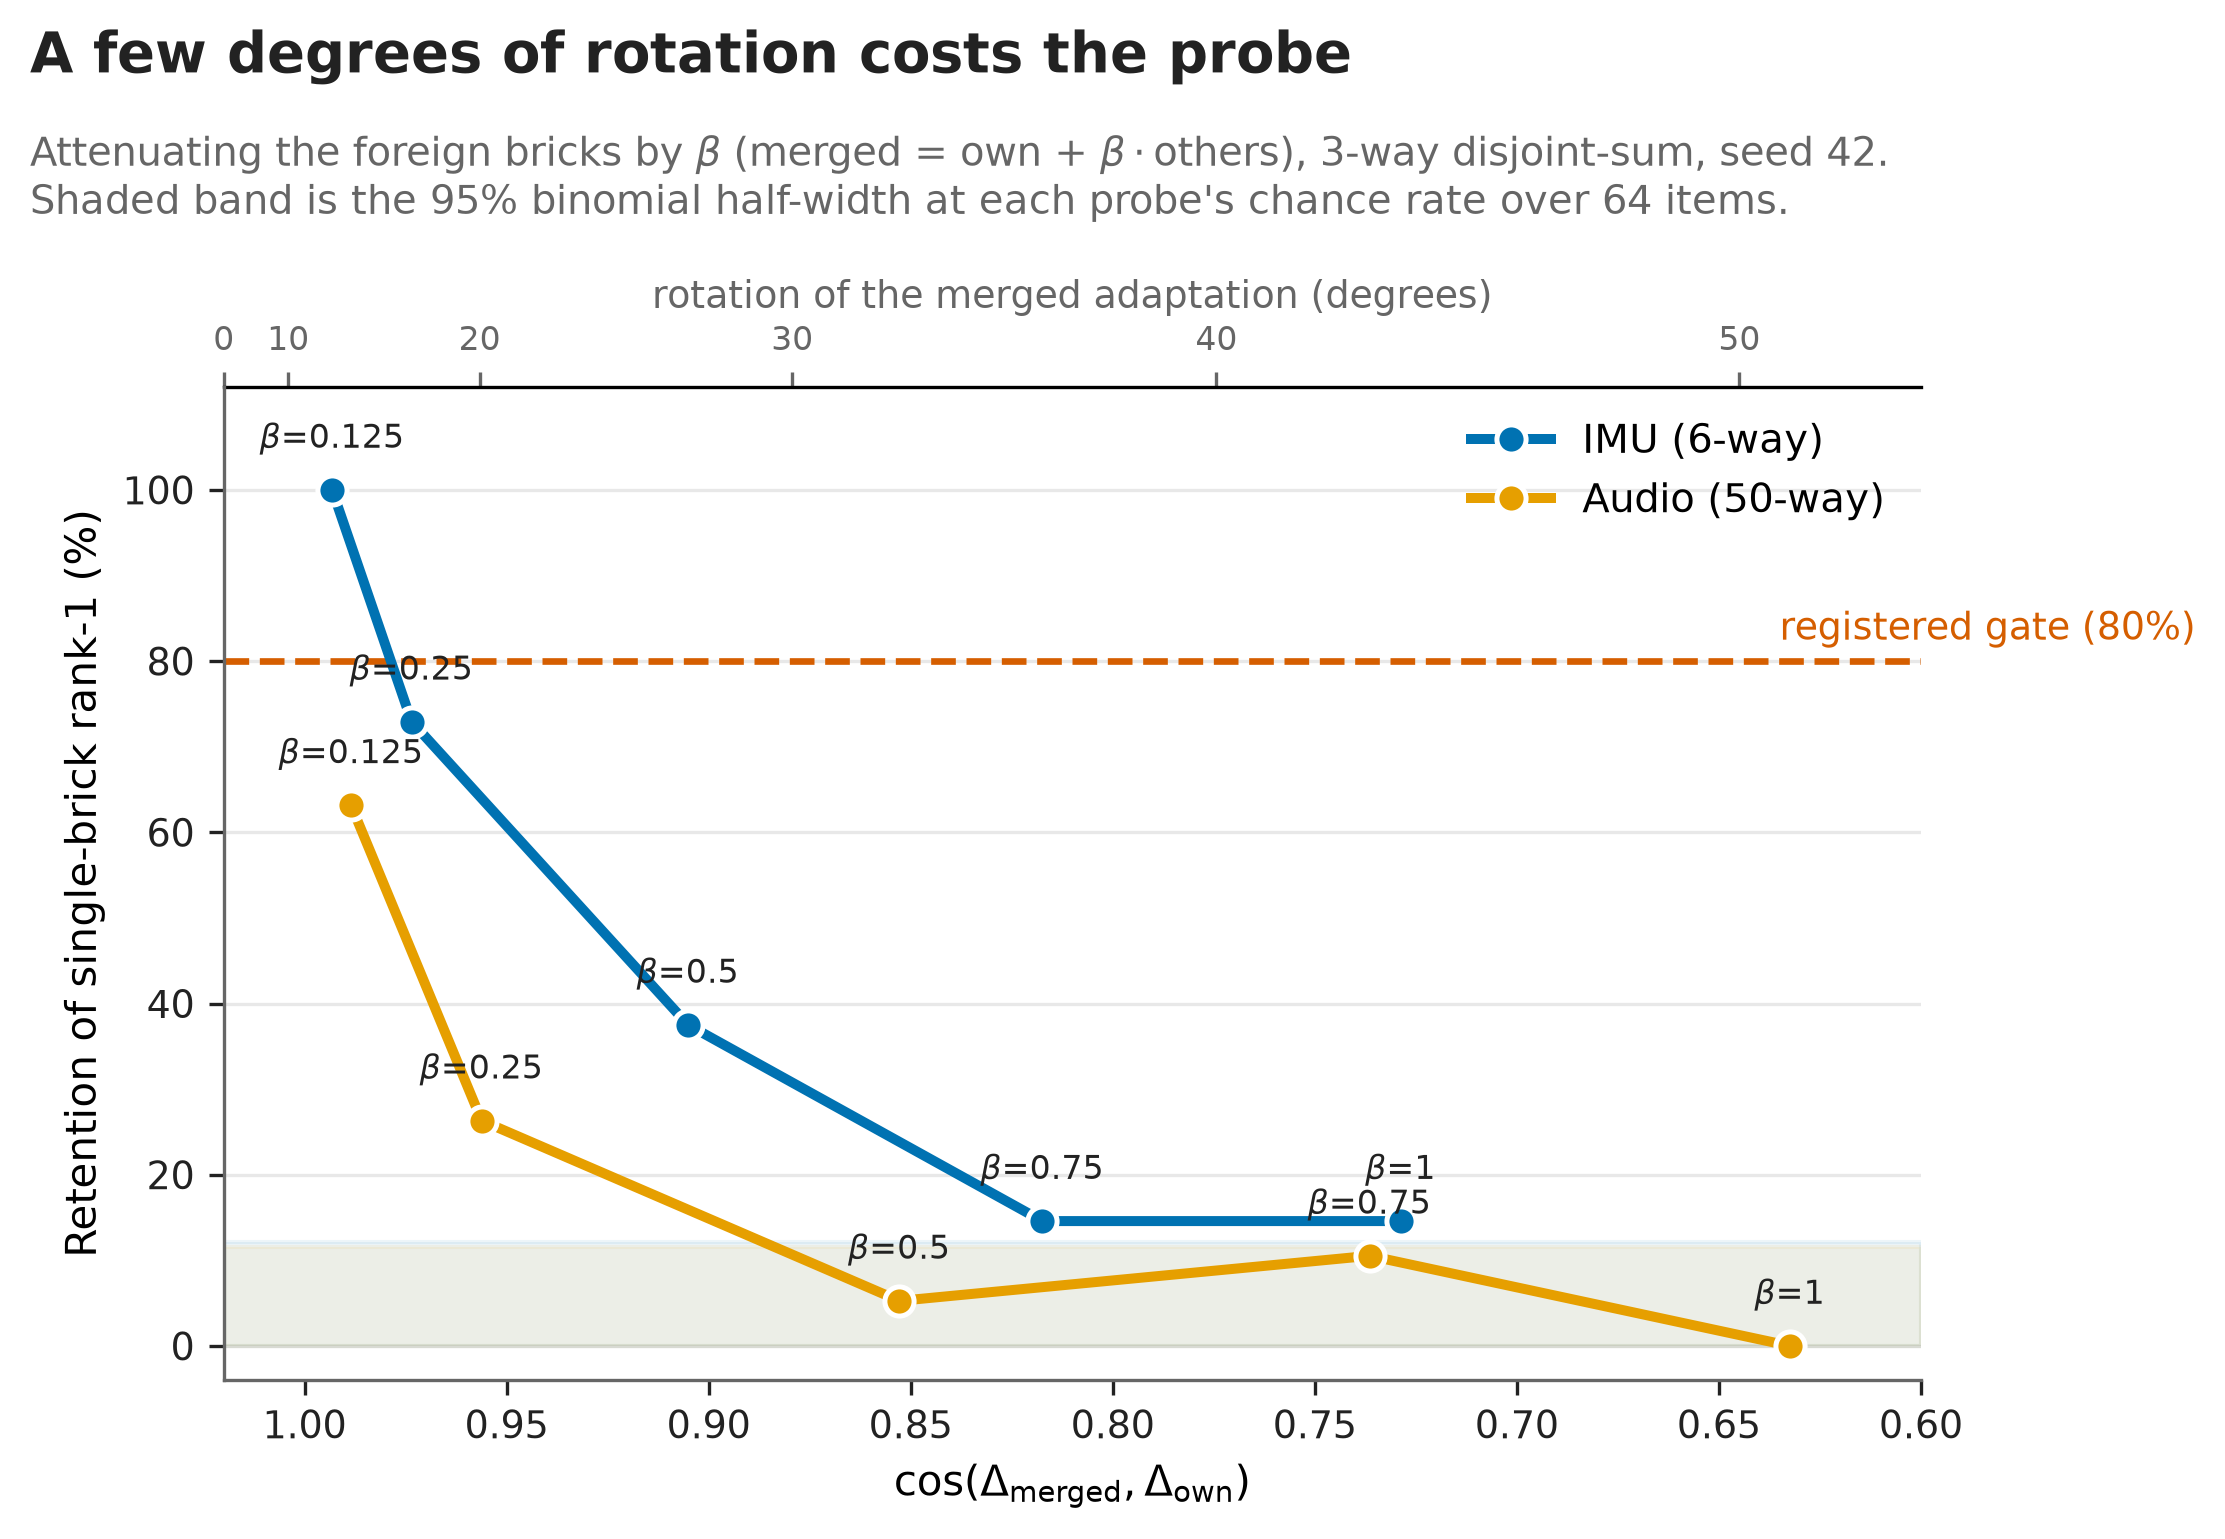
\includegraphics[width=0.82\linewidth]{paper7_dose_response.png}
\caption{The dose-response. Retention collapses within a few degrees of rotation: the registered 80\% gate is cleared only at $\cos \approx 0.99$, and only by the six-way probe. Shaded band is the 95\% binomial half-width at each probe's chance rate over 64 items.}
\label{fig:dose}
\end{figure}

\subsection{The sharpest cell: a powered probe erased}
Audio at 1800 steps is not a weak modality but a short-changed one: single-brick rank-1 rises from 0.078 to 0.328 against a 0.020 chance rate. Powered, it gives the starkest measurement in the paper. A brick that is right 19 times out of 64 on a fifty-way problem is right 0 times inside the three-way disjoint sum --- strictly worse than deleting it, since \texttt{others\_only} scores 0.016. The controls behaved throughout: \texttt{shuffled}, \texttt{random} and \texttt{no\_bridge} sit at chance in every single-brick column, so the instrument is sound and the failure is real.

\begin{figure}[t]
\centering
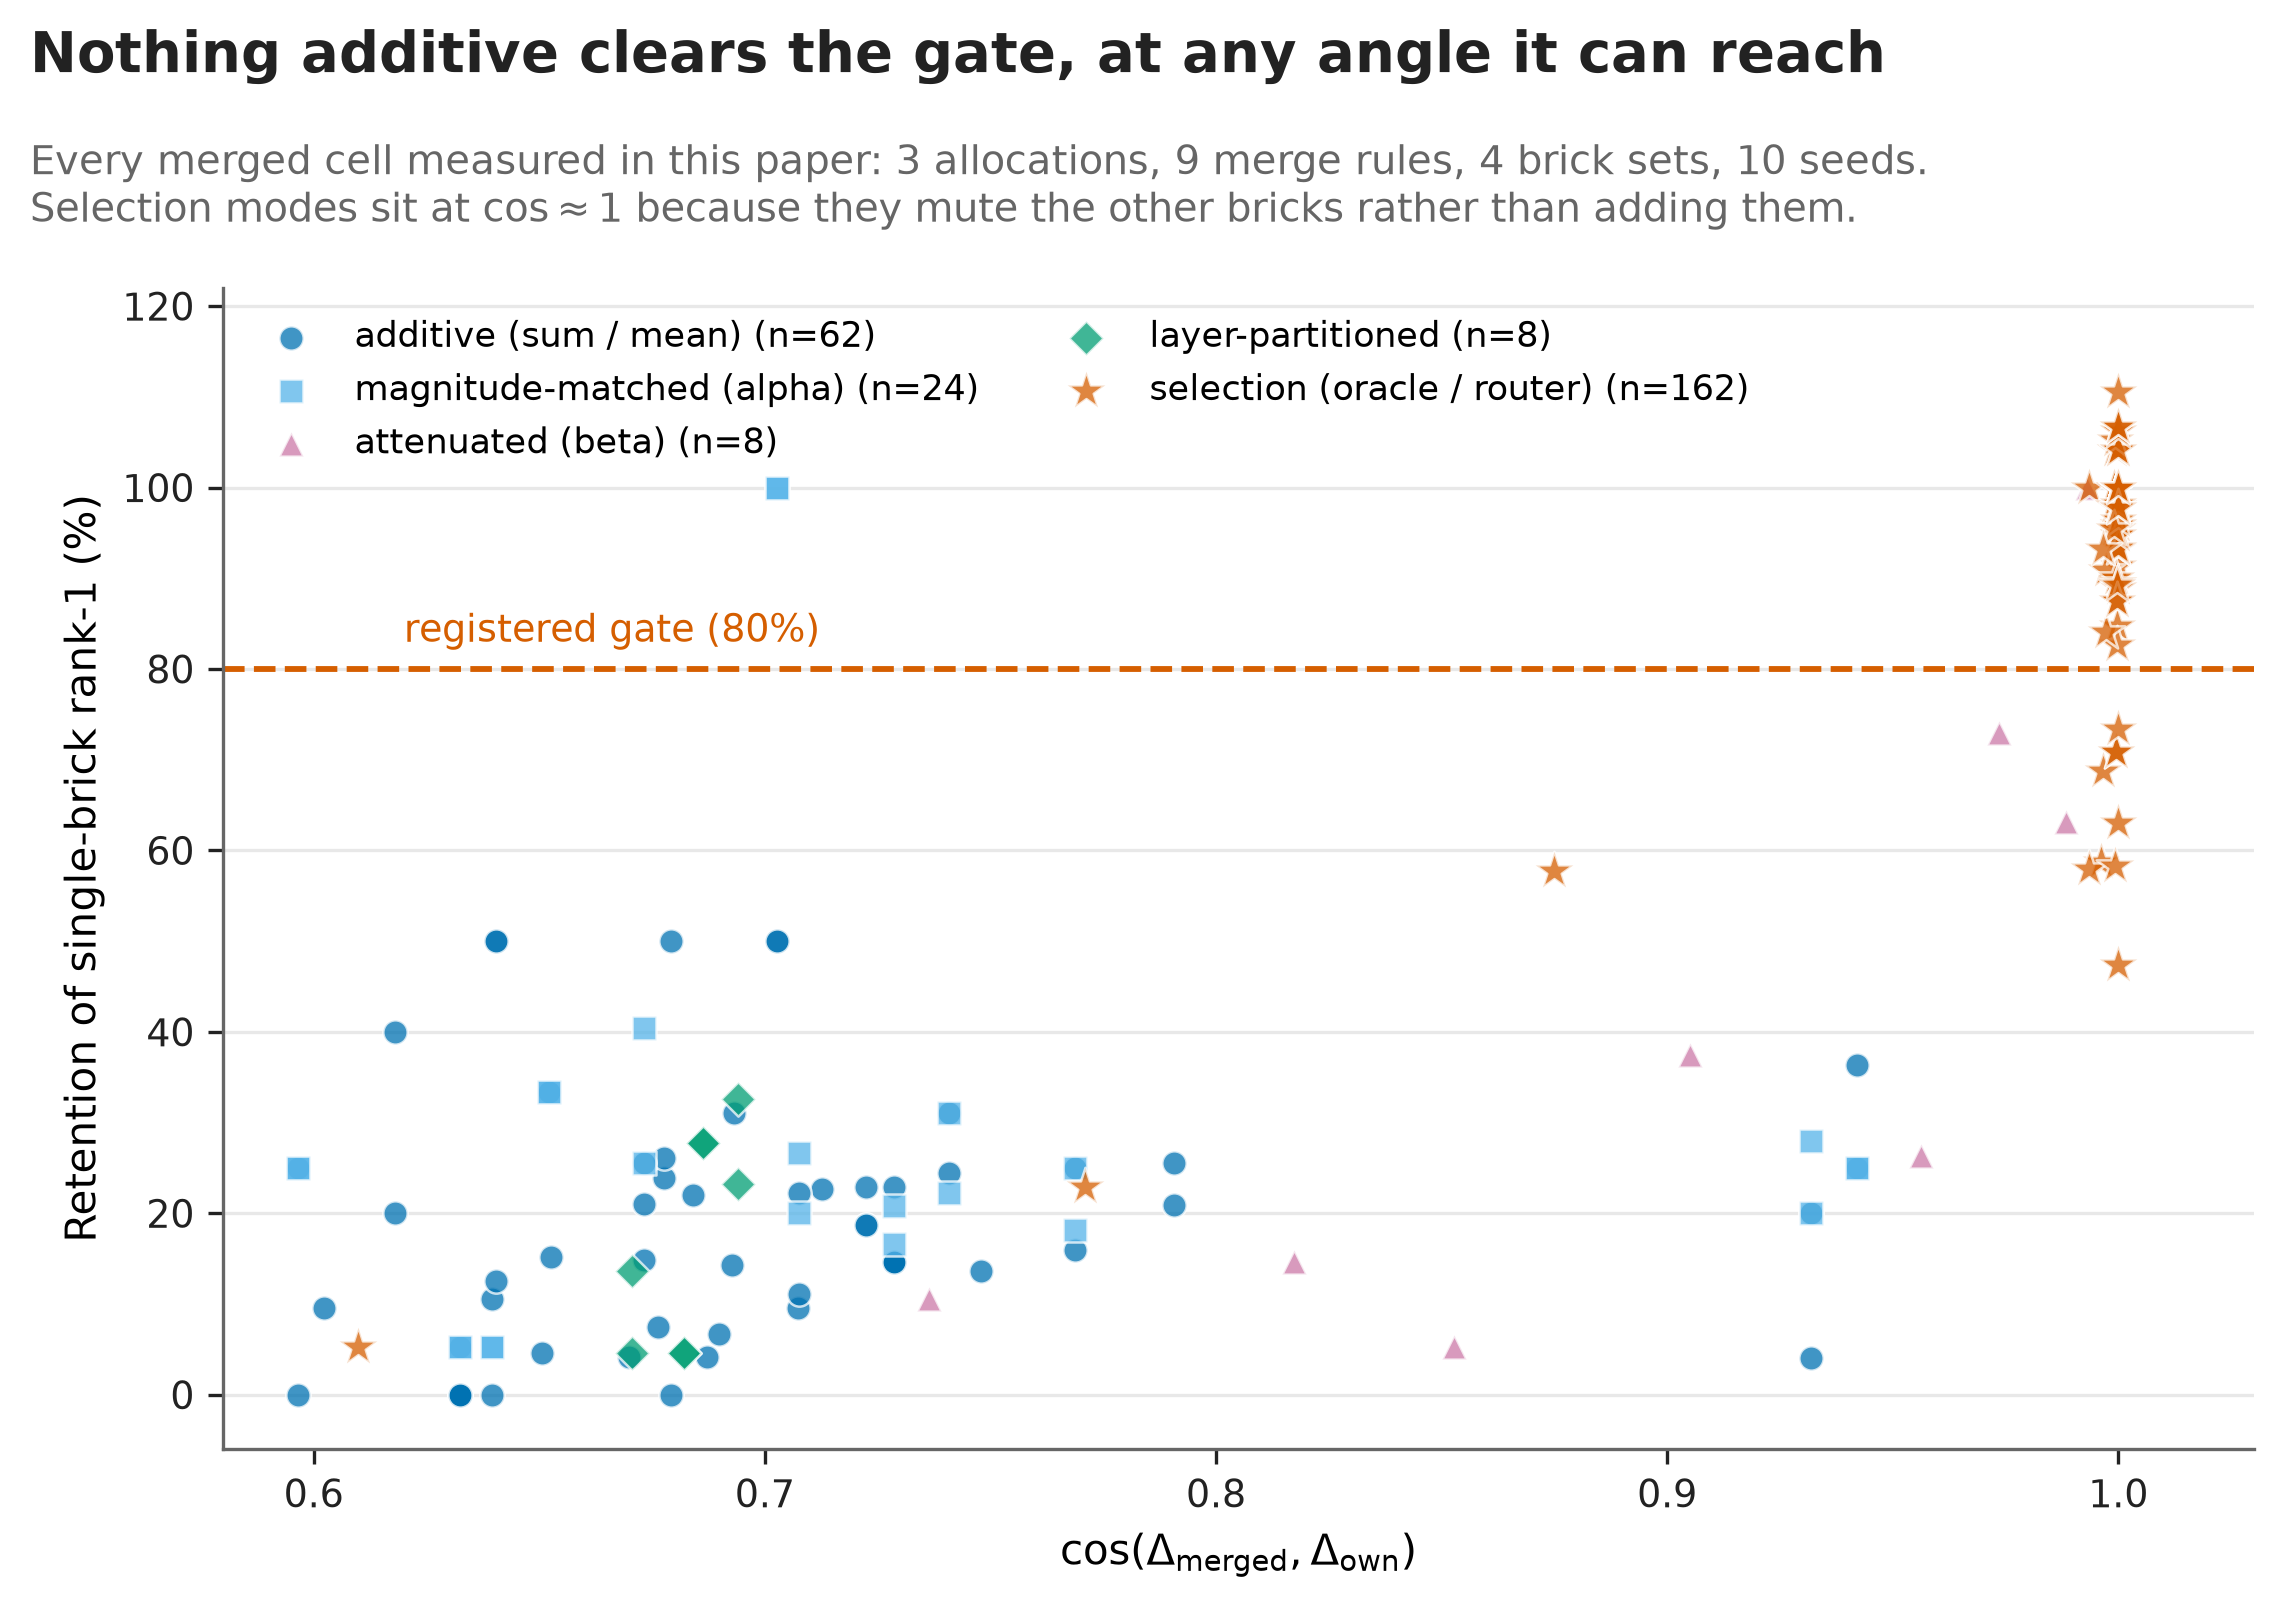
\includegraphics[width=0.9\linewidth]{paper7_retention_vs_cos.png}
\caption{Every merged cell in the paper, retention against $\cos(\mathrm{merged}, \mathrm{own})$, across allocations, merge rules, brick sets and seeds. The additive family occupies one region and one region only. Selection modes (stars at $\cos \approx 1$) are the only points above the gate, and the ones that fall below it are the collapsed router's cells.}
\label{fig:scatter}
\end{figure}

\section{Localizing the mechanism: a falsified prediction}
\label{sec:mechanism}
The dose-response invited an obvious inference: if $\cos = 1$ is the only survivable regime, build a design where $\cos = 1$ holds at every site a brick writes. Coefficient-space partitioning cannot do that --- the basis spans every LoRA site, so each brick is off-axis everywhere it writes --- but \emph{layer} partitioning can. The model has 14 decoder layers laid out layer-major in the flat vector, so a layer set is a contiguous flat range. The most equal contiguous three-way split is fixed by the architecture, not chosen: IMU layers 0--4 (272,384 dims, 35.2\%), audio layers 5--8 (229,376, 29.6\%), vision layers 9--13 (272,384, 35.2\%), each block holding exactly two of the six attention layers.

\paragraph{Registered prediction.}
The site-local angle account predicts $\sim$100\% retention, because $\cos(\mathrm{merged}, \mathrm{own})$ restricted to a brick's own block is $1.0$ by construction. The global angle account predicts retention at or below the phase-2 level. These differ by about 100 points, so the arm is decisive either way.

\paragraph{The geometry came out as designed.}
\begin{itemize}
  \item in-block $\cos(\mathrm{merged}, \mathrm{own}) = 0.9999999$ under both \texttt{sum} and \texttt{mean};
  \item \texttt{others\_in\_own\_block} $L_2 = 0.000e+00$ --- the other bricks put literally zero mass in the measured brick's sites;
  \item \texttt{own\_outside\_block} $L_2 = 0.000e+00$ --- and the measured brick puts literally zero mass outside them;
  \item coefficient recovery through the block basis at ratio 1.0000002, relative error 2.3e-07.
\end{itemize}
The control is clean: restricting a brick to a third of the sites costs almost nothing on its own --- IMU falls to 89.6\% of its full-layer single and audio \emph{rises} to 115.8\% at seed 42 (78.3\% and 104.8\% at seed 1042). A third of the sites is not a capacity bottleneck at these budgets, so whatever happens to the merged probes is not an artifact of the partition.

\paragraph{The prediction failed, and the failure replicates.}
Retention is 32.6\% (IMU) and 13.6\% (audio) at seed 42, and 27.8\% and 4.5\% at seed 1042 (Table~\ref{tab:layer}, Figure~\ref{fig:layer}). Every cell of both seeds fails the registered gate with all controls at chance. The \texttt{others\_only} control reproduces verbatim under this perfect geometry: at both seeds the merged score equals \texttt{others\_only} to within one evaluation item, and at seed 1042 the merged IMU score is \emph{below} it. A brick can own its sites outright --- perfect direction, perfect magnitude, provably zero foreign mass anywhere it writes --- and still lose its probe the moment two other bricks are switched on at \emph{other} layers.

The global-angle account is not rescued either: layer partitioning lands at global $\cos \approx 0.69$, where the dose curve predicts about 14.6\% for IMU, and observed retention is about twice that at seed 42 and level with it at seed 1042. Retention is therefore not a pure function of the global cosine either; the angle is a decent summary statistic \emph{within} a fixed allocation and does not transfer \emph{across} allocations.

What survives is the mechanism the failure implicates, and it should be stated in these words: \textbf{the damage is cross-layer residual-stream interaction, not weight-space overlap}. A probe reading out of the top of the stack runs its forward pass through every foreign adaptation installed anywhere along it, and that is enough to extinguish it. Disjoint sites do not protect a probe, because the interference is downstream of the sites.

Whether layer partitioning helps \emph{at all} is not resolved by two seeds and is not claimed. Against the matched full-layer comparator at seed 42 IMU goes 14.6\% $\to$ 32.6\% and audio 0.0\% $\to$ 13.6\%, which looks like a doubling; at seed 1042 the comparison is 15.2\% against 27.8\%, which is indistinguishable. The defensible statement is that layer partitioning is at best a modest improvement, inside seed spread, and nowhere near the $\sim$100\% its own prediction required.

\begin{table}[t]
\centering
\caption{The layer-partition falsification, both seeds. Each brick owns its sites exactly --- in-block $\cos = 1$, zero foreign mass in-block --- and the probe dies anyway, landing on \texttt{others\_only}. ``Full-layer single'' is the same brick trained at the same budget and seed without the site restriction.}
\label{tab:layer}
\footnotesize
\begin{tabular}{llrrrrrrr}
\toprule
Seed & Probe & Full-layer & Restricted & In-block $\cos$ & Foreign in-block & Merged & Retention & \texttt{others\_only} \\
 & & single & single & & $L_2$ & (sum) & & \\
\midrule
42 & imu & 0.750 & 0.672 & 0.9999999 & 0.000e+00 & 0.219 & 32.6\% & 0.203 \\
42 & audio & 0.297 & 0.344 & 0.9999999 & 0.000e+00 & 0.047 & 13.6\% & 0.047 \\
1042 & imu & 0.719 & 0.562 & 1.0000001 & 0.000e+00 & 0.156 & 27.8\% & 0.172 \\
1042 & audio & 0.328 & 0.344 & 1.0000000 & 0.000e+00 & 0.016 & 4.5\% & 0.016 \\
\bottomrule
\end{tabular}
\end{table}

\begin{figure}[t]
\centering
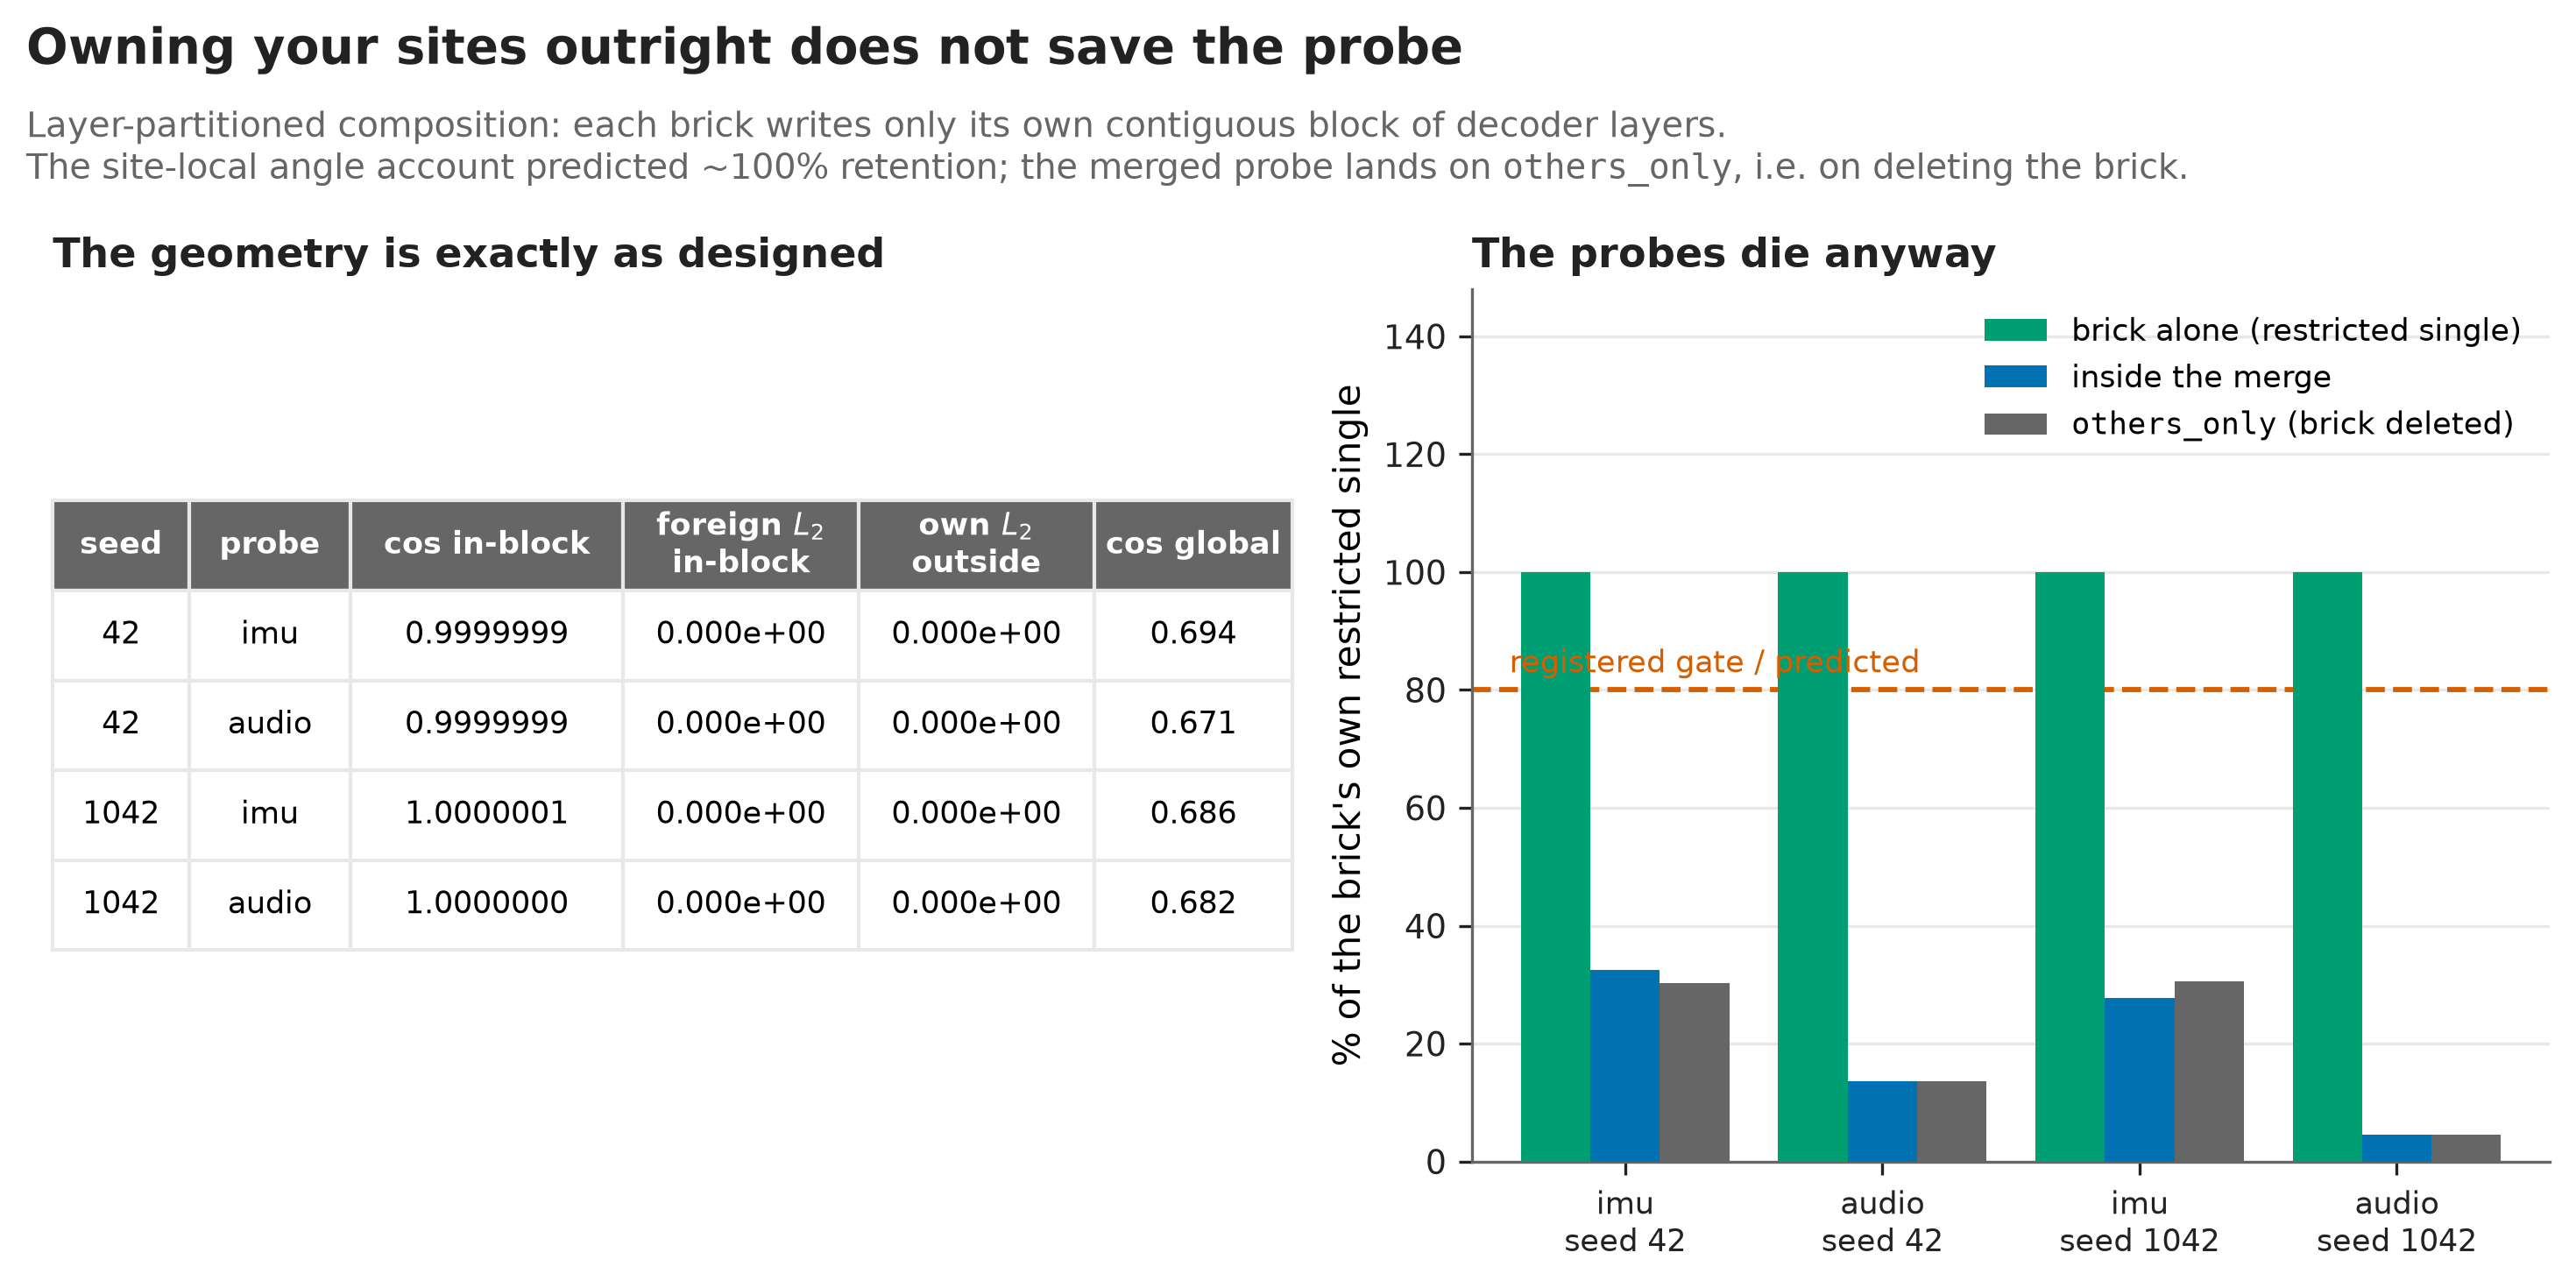
\includegraphics[width=0.92\linewidth]{paper7_layer_partition.png}
\caption{The falsification in one panel. Left: the weight-space geometry is exactly as designed at both seeds. Right: the probes die anyway, landing on the \texttt{others\_only} control, roughly 70--95 points below the prediction the geometry licensed.}
\label{fig:layer}
\end{figure}

\section{Selection, stated honestly}
\label{sec:selection}

\subsection{The ceiling is exact and the feature-only null is provably blind}
Routing each probe through only its own brick's weights --- a hard one-hot oracle over the coefficient heads --- reproduces the single-brick number exactly: retention 1.000 in both modalities at all 8 seeds, 16 cells of 16, with $\cos(\mathrm{merged}, \mathrm{own}) = 1$ and $\|\mathrm{merged}\| = \|\mathrm{own}\|$. This is a ceiling, not a result, but it settles what the whole negative family left open: \textbf{composition under this architecture is solvable}. Having three bridges loaded damages no brick. Every point of loss in \S\ref{sec:negative} and \S\ref{sec:mechanism} is attributable to \emph{adding the other bricks in}, and a mechanism that declines to add them recovers 100\% of both modalities.

The complementary null is equally emphatic. Our gate protocol is leak-free by construction: the live slot and the ambient slots are drawn from the \emph{same} per-brick pool, so a router that sees only the concatenated sensor features has the same input distribution whichever modality is being asked. It therefore has no input-conditioned solution, and the measurement confirms the argument mechanically --- the feature-only router's between-modality $L_1$ gap is 0.000e+00 at every one of the 8 seeds, byte-identical gate vectors whichever brick owns the question, while its within-modality dispersion is nonzero. It is not a frozen constant; it is \emph{modality-blind}. That is the correct answer to the question it was asked, which means the earlier collapse of feature-conditioned routers was never an optimizer failure, and it means the only informative router in this family is a task-conditioned one.

For completeness, Table~\ref{tab:collapse} shows the feature-conditioned family swept over load-balancing weight and router learning rate. Load balancing only chooses \emph{which} brick the constant lands on; lowering the learning rate only slides the constant from one-hot toward uniform, and a uniform gate \emph{is} the mean merge. The apparent 100\% IMU cells are accidents of the constant pointing at IMU, which is exactly why the roll-up gate requires every modality to clear.

\begin{table}[t]
\centering
\caption{The feature-conditioned router family, seed 42 (single seed). ``Gate mass'' is the mean convex weight over (imu, audio, vision); the $L_1$ gap is between the two measured modalities' mean gate vectors. Every row is a constant: the gap is at the numerical floor, so no row routes.}
\label{tab:collapse}
\small
\begin{tabular}{lrrrr}
\toprule
Router & Gate mass (imu, audio, vision) & Between-modality $L_1$ & IMU ret. & Audio ret. \\
\midrule
$\lambda = 0$ & 1.000, 0.000, 0.000 & 0.0e+00 & 100.0\% & 15.8\% \\
$\lambda = 0.5$ & 1.000, 0.000, 0.000 & 0.0e+00 & 100.0\% & 15.8\% \\
$\lambda = 2$ & 1.000, 0.000, 0.000 & 0.0e+00 & 100.0\% & 15.8\% \\
$\lambda = 8$ & 0.000, 1.000, 0.000 & 0.0e+00 & 29.2\% & 100.0\% \\
router lr $1\times$ & 0.897, 0.001, 0.102 & 0.0e+00 & 70.8\% & 10.5\% \\
router lr $0.1\times$ & 0.851, 0.056, 0.094 & 0.0e+00 & 68.8\% & 5.3\% \\
router lr $0.01\times$ & 0.429, 0.364, 0.207 & 0.0e+00 & 22.9\% & 5.3\% \\
\bottomrule
\end{tabular}
\end{table}

\subsection{The task-conditioned router reaches the ceiling --- in 6 seeds of 8}
Given a learned embedding of \emph{which task is being asked}, the router can in principle route. At seed 42 it looked like a clean pass: five of six grid cells cleared the gate in both modalities. The registered replicate at seed 1042 \textbf{reversed} it: zero of six. That split changed the reportable quantity from ``does it pass'' to ``how often does it escape'', and eight seeds were run in total at an identical six-cell grid (router learning rate $\in \{0.3, 1, 3\} \times$ the bridge rate, with and without an entropy bonus). Table~\ref{tab:escape} and Figure~\ref{fig:escape} report every seed; none is dropped.

The escape rate is \textbf{6/8}. The two outcomes are close to bimodal rather than a continuum: escaped seeds land with \texttt{load\_ema} at $\approx$ [0.53, 0.46, 0.01] over (imu, audio, vision) and own-brick mass 0.85--1.00 on audio; collapsed seeds land at $\approx$ [0.85, 0.003, 0.15] with audio's own mass at 0.002--0.005. Only one seed sits between the modes, so the paper says ``close to bimodal'' rather than claiming a clean switch from eight points.

Three facts locate the failure in the training dynamic rather than in the configuration.

\begin{enumerate}
  \item \textbf{The grid does not decide it.} No cell is safe across seeds and none fails across seeds: the best cells (\texttt{gate-task-lr-3}, \texttt{gate-task-lr-1-ent0.1}) clear 6/8 overall and 6/6 among the escaped seeds; the worst clear 4/8. The grid moves the result by a cell or two; the seed moves it by six.
  \item \textbf{The bricks do not decide it.} The collapsing seeds have audio bricks that are, if anything, better (0.328, 0.328 against seed 42's 0.297), and the oracle reaches 100\% at every seed.
  \item \textbf{The failure has a direction.} It is always audio that is starved. Across the collapsed seeds' task-conditioned cells, IMU retention stays at 63.0--100.0\% while audio falls to 0.0--9.5\%. The router collapses onto the brick whose language-model loss moves most. Task conditioning weakens that attractor enough to escape it most of the time; it does not remove it.
\end{enumerate}

The entropy bonus does not fix it: at the collapsing seeds it raises per-example routing entropy and still routes to IMU in both modalities --- softmax temperature without separation --- and at seed 42 it was actively harmful at the highest learning rate, producing that seed's only failing task-conditioned cell.

What the escaped seeds show is worth keeping, because it is exact. When the router engages, $\cos(\mathrm{merged}, \mathrm{own}) = 1.0000$ and $\|\mathrm{merged}\| = 52.59$ against $\|\mathrm{own}\| = 52.59$, with retention at or above 100\% in both modalities. The router does not find a better way to \emph{add} the bricks; it \textbf{mutes} them, returning the merged delta to the $\cos \approx 1$ regime the dose-response identified as the only survivable one. The dose curve, the oracle, and the escaped router are three views of one fact. (Retention above 100\%, up to 110.5\%, is noise: one item is 1.6 points and a near-one-hot mixture differing by two items sits well inside that. The claim is ``recovers the single-brick number'', not ``beats it''.)

\begin{table}[t]
\centering
\caption{Router escape across 8 seeds at an identical six-cell grid. ``Cells clearing'' counts task-conditioned cells that clear 80\% in \emph{every} measured modality. \texttt{load\_ema} and own-brick mass are read at \texttt{gate-task-lr-1}. No seed is dropped.}
\label{tab:escape}
\footnotesize
\begin{tabular}{lrlrrl}
\toprule
Seed & Cells clearing & \texttt{load\_ema} (imu, audio, vision) & Own mass (IMU) & Own mass (audio) & Outcome \\
\midrule
42 & 5/6 & 0.499, 0.489, 0.012 & 1.000 & 0.983 & escaped \\
1042 & 0/6 & 0.883, 0.005, 0.113 & 0.992 & 0.005 & \textbf{collapsed} \\
2042 & 6/6 & 0.498, 0.493, 0.009 & 0.999 & 0.998 & escaped \\
3042 & 0/6 & 0.811, 0.002, 0.187 & 0.968 & 0.002 & \textbf{collapsed} \\
4042 & 6/6 & 0.500, 0.496, 0.004 & 1.000 & 0.991 & escaped \\
5042 & 4/6 & 0.675, 0.307, 0.018 & 0.995 & 0.848 & escaped \\
6042 & 5/6 & 0.497, 0.502, 0.001 & 1.000 & 0.999 & escaped \\
7042 & 4/6 & 0.505, 0.493, 0.003 & 1.000 & 1.000 & escaped \\
\midrule
\multicolumn{5}{l}{\textbf{Escape rate}} & \textbf{6/8 seeds} \\
\bottomrule
\end{tabular}
\end{table}

\begin{figure}[t]
\centering
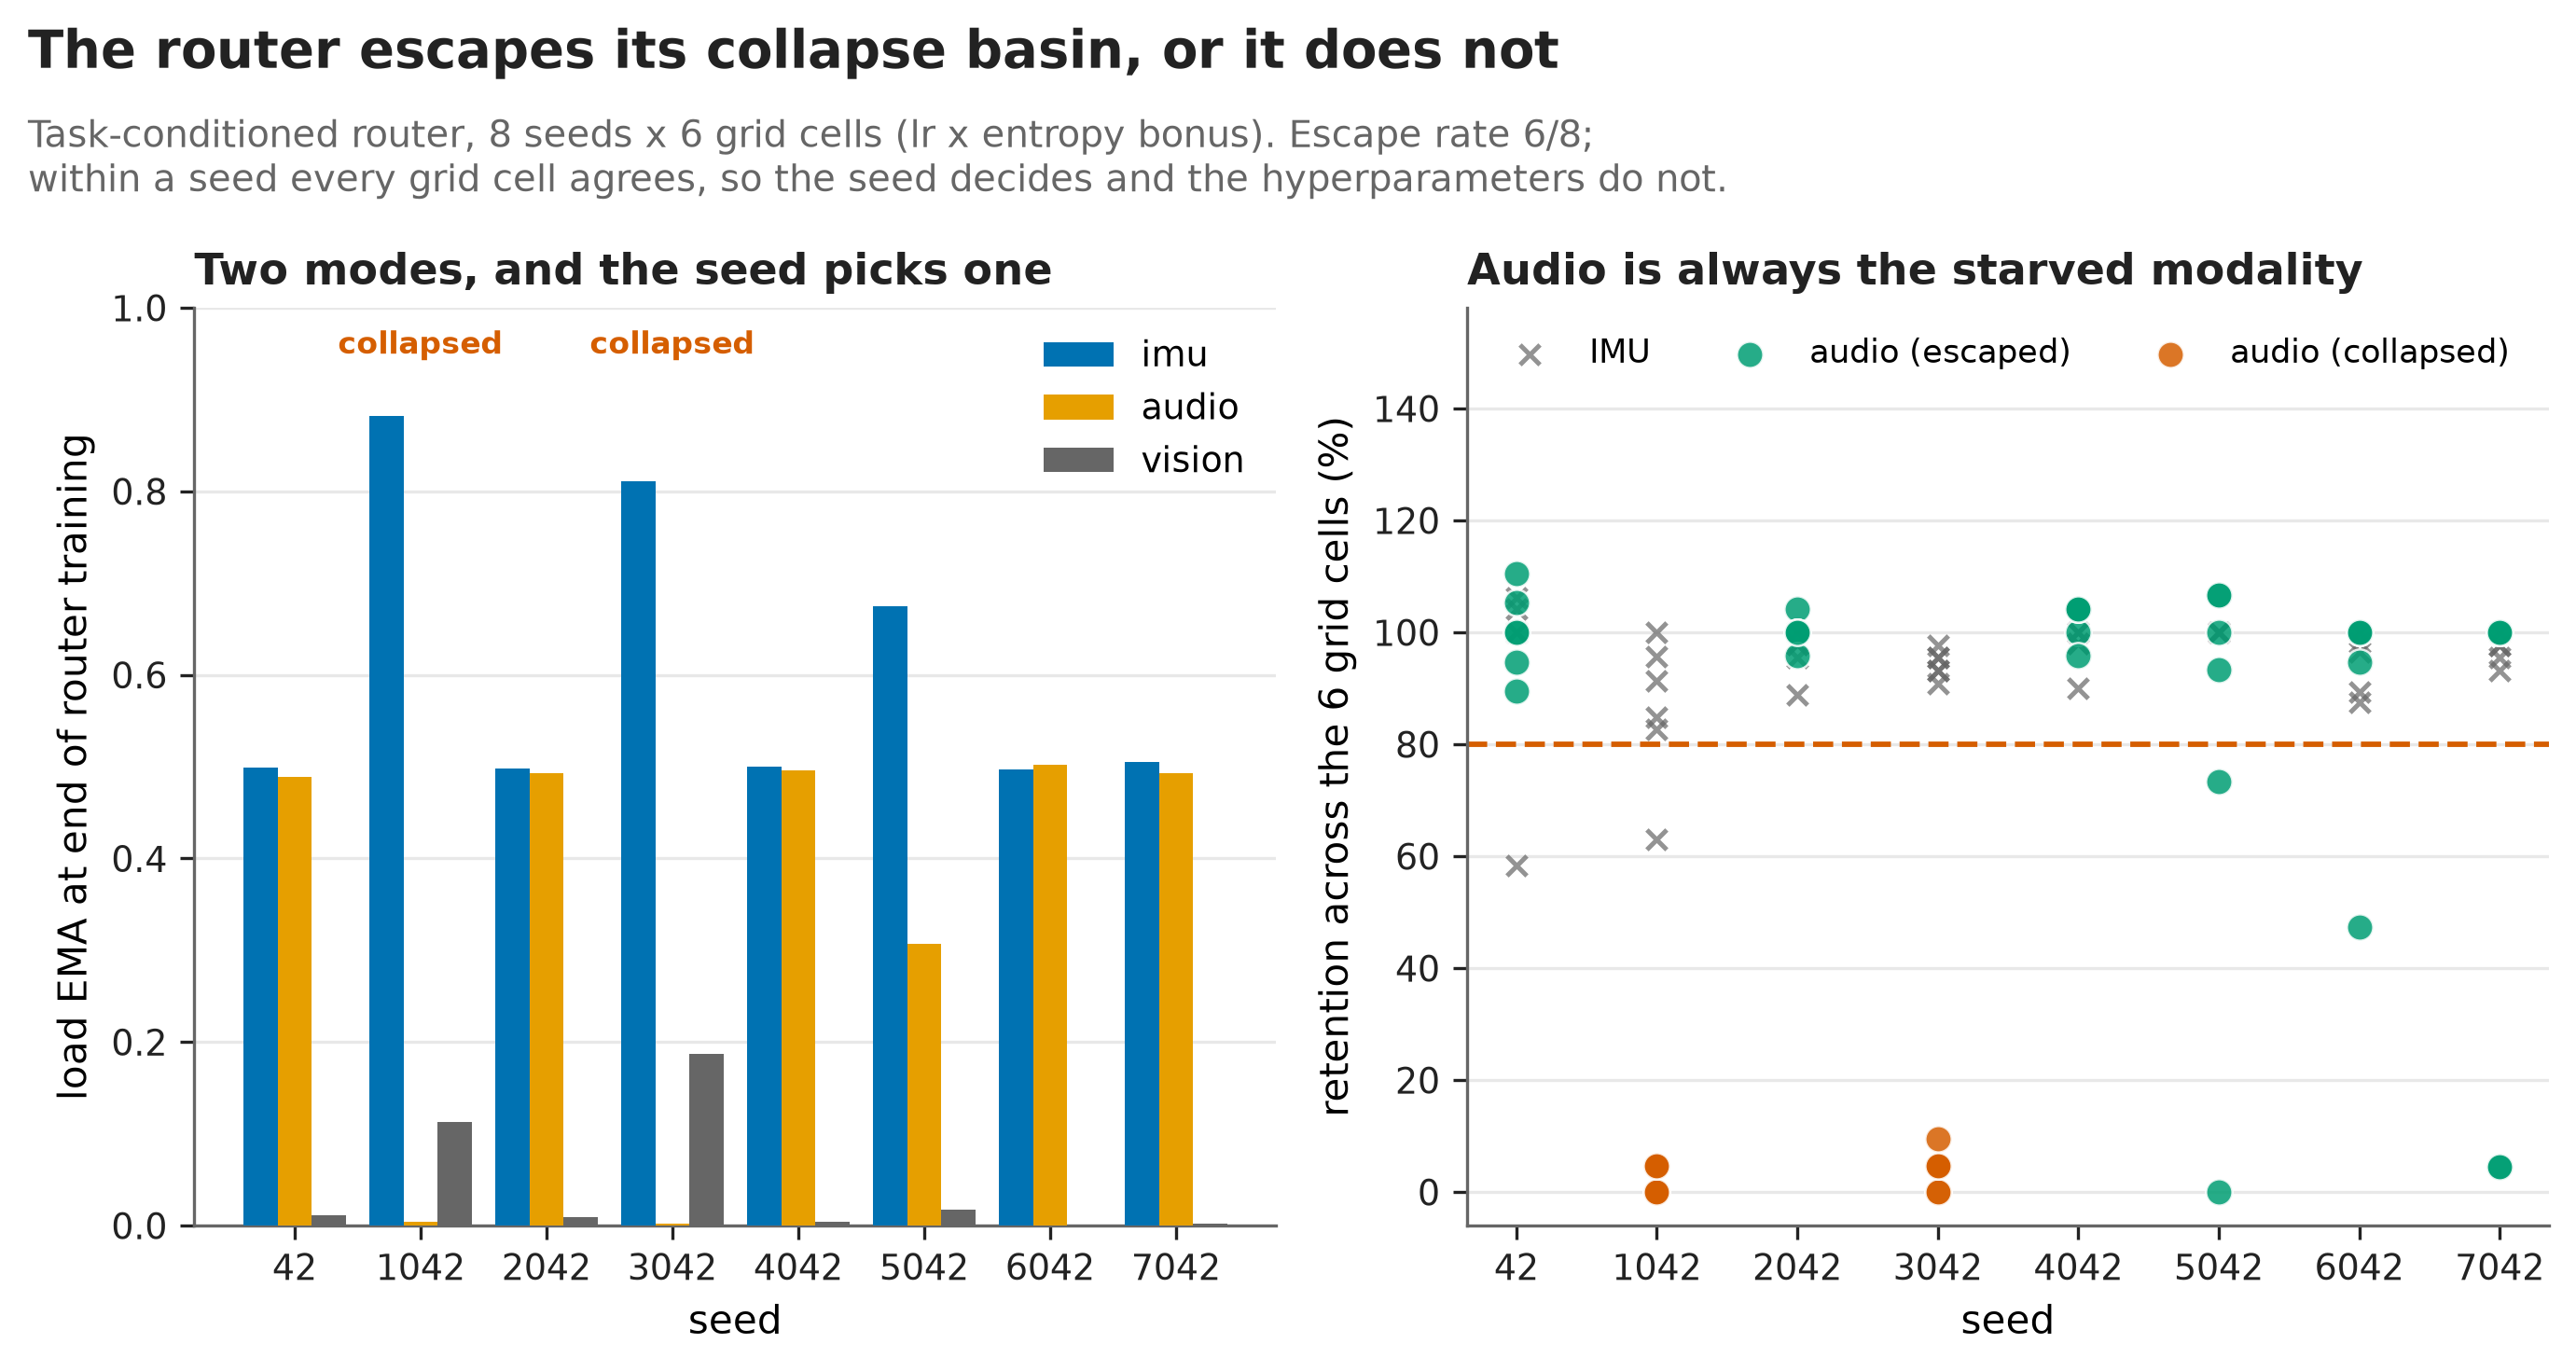
\includegraphics[width=0.9\linewidth]{paper7_router_escape.png}
\caption{The escape is close to bimodal and hyperparameter-independent. Left: end-of-training load EMA per seed --- either the router splits its load between the two task bricks, or it collapses onto IMU. Right: retention of both probes across all six grid cells of each seed; IMU survives everywhere, audio is either recovered or extinguished, and the cells within a seed agree.}
\label{fig:escape}
\end{figure}

\subsection{Two caveats that must travel together}
\textbf{First, the router is \emph{given} the task identity.} It still has to learn, from the language-model loss alone with no supervision on brick identity, that this identity maps to a near-one-hot selection over coefficient heads --- and when it escapes, it does, in 600 steps. But it should be described for what it is: a \emph{learned oracle}, not a system that infers from the sensor stream which brick is relevant. Under this construction the sensor stream \emph{cannot} carry that signal, by design, and the modality-blind null proves it at all 8 seeds with a between-modality $L_1$ gap of 0.000e+00.

\textbf{Second, it fails outright in a quarter of the seeds, and nothing in the grid predicts which.} A mechanism that reaches the ceiling on 6 seeds and chance on 2, with no hyperparameter selecting between them, is a result --- but it is not yet a method.

So the honest form: \textbf{selection-based composition is exactly right when it engages, recovering each brick's single-brick probe to the item, and the only learned mechanism we found for engaging it collapses onto the loudest brick in 2 seeds of 8}. This section is an existence proof plus a named open problem, not a recipe. Anything stronger would be a claim built on a seed --- which is exactly what the seed-42 run would have supported and the seed-1042 run refuted.

\section{The open problem}
\label{sec:open}
Addition is closed. Every additive rule we can construct fails, including the two that were designed to be interference-free by construction, and the mechanism is now localized somewhere addition cannot reach. Routing is the road, and the specific obstacle is not architectural but dynamical: \textbf{make the router's escape selectable}. The escape is bimodal, hyperparameter-independent and directional --- it collapses onto the brick whose loss moves most --- which points at the optimization schedule rather than the architecture. Three concrete candidates: per-brick loss normalization, so no expert can win the race to saturation; a warmup in which each expert is trained alone before the router is allowed to mix; and explicit routing supervision, which trades the ``learned'' claim for a working system and would establish the upper bound the unsupervised version is chasing. A second open question follows immediately from the collapse mechanism: the escape rate should degrade with the number of experts, so three or four probed modalities is the test that says whether 6/8 is a floor or a ceiling.

\section{Related Work}
Weight-space merging is a mature literature that this paper's instrument reads differently. Task arithmetic \cite{ilharco2023task} composes fine-tuned models by adding task vectors; TIES-merging \cite{yadav2023ties} resolves sign conflicts and trims low-magnitude entries before summing; DARE \cite{yu2024dare} shows delta parameters are extremely redundant and rescales after random dropping; model soups \cite{wortsman2022soups} average weights of models fine-tuned from a common initialization. LoRA-specific composition includes LoraHub \cite{huang2024lorahub}, which learns per-task mixing coefficients over a library of adapters. All of these report in-objective or aggregate downstream metrics --- average accuracy over a task set, or the merged model's score on each task's own benchmark. Our contribution is orthogonal to the merge rules and lies in the measurement: \emph{each constituent's own behavioral probe, re-measured under the merge, against an \texttt{others\_only} control}. That instrument is what converts ``retention is 94.7\%'' into ``the probe is at chance'', and it is what makes the disjoint-allocation negative interpretable rather than merely disappointing.

The interference we measure is also distinct from what the merging literature usually models. TIES and DARE both treat interference as a \emph{parameter-space} phenomenon --- sign disagreement and magnitude swamping in shared coordinates --- and both mitigate it by editing coordinates. Our disjoint and layer allocations remove that phenomenon entirely, by construction and by measurement, and the behavioral damage survives unchanged, which localizes it downstream in the residual stream.

The routing half connects to mixture-of-experts. Sparse expert routing and its load-balancing pathologies are well documented \cite{shazeer2017moe,fedus2022switch}: a router that collapses onto a subset of experts, starving the rest, is the classical imbalance failure, and the standard remedy is an auxiliary load-balancing loss. We observe exactly that pathology in an unusual setting --- three experts, two tasks, a router over \emph{adapter coefficient heads} rather than over feed-forward blocks --- and we report that the standard remedy does not work here: the balance penalty pinned within 1\% of its theoretical maximum only chooses \emph{which} expert the constant lands on. What does work, when it works, is conditioning the router on task identity, which is closer to the per-task mixing of LoraHub than to per-token MoE routing; and what remains open is the bistability, which the MoE literature's expert-choice and warmup remedies are the natural next place to look.

Finally, the conditional bridge itself and its basis reparameterization are prior work of ours \cite{penov2026bridges,penov2026note,penov2026basis}; the composition negative reported at the end of \cite{penov2026basis} is what this paper set out to fix.

\section{Limitations}
\textbf{One model, one scale.} Every number is on LFM 2.5 230M. ``Six degrees of rotation costs you the probe'' is exactly the sort of claim that could soften with model size, and no scale point above 230M is reported here.
\textbf{Two probed bricks.} Routing over two task bricks plus one context brick is the easiest routing problem that is not trivial, and n = 2 turns out to be bistable; the paper does not overclaim from it.
\textbf{Vision is never probed.} The suite has no vision label probe, so vision enters as a context brick trained on the text objective and is measured only through the damage it does. All behavioral claims are scoped to IMU and to audio at 1800 steps.
\textbf{64 evaluation items per probe.} One item is 1.6 points and the 95\% binomial half-width at the six-way chance rate is $\pm0.091$; differences below about five points are not resolvable, and no ranking is claimed inside that band.
\textbf{Single-seed cells.} The dose-response curve, the pairwise decomposition, the four-merge-rule table and the collapsed-router family are seed 42 only, and are labelled as such wherever they appear. The three-seed and eight-seed aggregates carry the load-bearing claims.
\textbf{The layer partition is contiguous and balanced by flat size.} Interleaved and capacity-matched partitions are unexplored; what is falsified is the pure-angle prediction, not every conceivable site partition.
\textbf{The router is task-conditioned and its escape is seed-determined.} See \S\ref{sec:selection}; these two caveats are load-bearing and neither can be dropped.

\section{Conclusion}
We built the measurement that composition research is missing --- each constituent's own out-of-objective probe under the merged weights --- and it changes what the results say. A merge that is provably lossless in weight space, verified to a coefficient recovery ratio of 1.000006, is behaviorally dead; a merge that scores 94.7\% on the in-objective metric is dead in exactly the same way. The tolerance for adding a foreign adaptation is about 7 degrees, so no additive rule survives, and when we built the one design our own angle account said should work --- perfect ownership of disjoint sites --- it failed at two seeds, which localizes the damage as cross-layer residual-stream interaction rather than weight-space overlap. What does work is not arithmetic but selection: an oracle recovers every brick exactly at every seed, and a task-conditioned learned router reaches that ceiling precisely when it escapes a collapse basin, in 6 seeds of 8. The headline is the one the whole paper is built around: \textbf{zero weight-space interference is not enough}. The next problem is not a better merge rule; it is making the escape selectable.

\section*{Reproducibility Statement}
Every number in this manuscript is rendered from the bundled run artifacts by the repository's renderer (\texttt{src/render\_arxiv7.py}); the figures are rendered from the same artifacts by \texttt{src/figures7.py}. The artifacts in \texttt{arxiv7/artifacts/} are the raw per-run JSON written by the harness, and the same files drive the per-run reports produced by \texttt{python -m src.report\_disjoint}, so the manuscript and the run reports cannot disagree. Editing \texttt{arxiv7/main.tex} by hand is reverted on the next render. Code, artifacts, and the exact render pipeline: \url{https://github.com/kortexa-ai/legolm.basis}.

\bibliographystyle{plain}
\bibliography{references}
\end{document}
